%%
%% Automatically generated file from DocOnce source
%% (https://github.com/doconce/doconce/)
%% doconce format html testdoc.do.txt --examples_as_exercises --latex_code_style=default:lst-blue1[style=myspeciallststyle,numbers=left,numberstyle=\tiny,stepnumber=3,numbersep=15pt,xleftmargin=1mm]@fcod:vrb-gray@sys:vrb[frame=lines,label=\fbox{{\tiny Terminal}},framesep=2.5mm,framerule=0.7pt] --latex_code_lststyles=mylststyles --latex_packages=varioref
% #define PREAMBLE
% #ifdef PREAMBLE
%-------------------- begin preamble ----------------------
\documentclass[%
oneside,                 % oneside: electronic viewing, twoside: printing
final,                   % draft: marks overfull hboxes, figures with paths
10pt]{article}
\listfiles               %  print all files needed to compile this document
\usepackage{relsize,makeidx,color,setspace,amsmath,amsfonts,amssymb}
\usepackage[table]{xcolor}
\usepackage{bm,ltablex,microtype}
\usepackage[pdftex]{graphicx}
\usepackage{sidecap}
% user-provided packages: --latex_packages=varioref
\usepackage{varioref}
% 'on page ...' reference with \vref{} and varioref package
\renewcommand\reftextfaceafter{on page~\thevpagerefnum}
\renewcommand\reftextfacebefore{on page~\thevpagerefnum}
\renewcommand\reftextafter{on page~\thevpagerefnum}
\renewcommand\reftextbefore{on page~\thevpagerefnum}
% Tools for marking corrections
\usepackage{soul}
\newcommand{\replace}[2]{{\color{red}\text{\st{#1} #2}}}
\newcommand{\remove}[1]{{\color{red}\st{#1}}}
% Packages for typesetting blocks of computer code
\usepackage{fancyvrb,framed,moreverb}
% Define colors
\definecolor{orange}{cmyk}{0,0.4,0.8,0.2}
\definecolor{tucorange}{rgb}{1.0,0.64,0}
\definecolor{darkorange}{rgb}{.71,0.21,0.01}
\definecolor{darkgreen}{rgb}{.12,.54,.11}
\definecolor{myteal}{rgb}{.26, .44, .56}
\definecolor{gray}{gray}{0.45}
\definecolor{mediumgray}{gray}{.8}
\definecolor{lightgray}{gray}{.95}
\definecolor{brown}{rgb}{0.54,0.27,0.07}
\definecolor{purple}{rgb}{0.5,0.0,0.5}
\definecolor{darkgray}{gray}{0.25}
\definecolor{darkblue}{rgb}{0,0.08,0.45}
\definecolor{darkblue2}{rgb}{0,0,0.8}
\definecolor{lightred}{rgb}{1.0,0.39,0.28}
\definecolor{lightgreen}{rgb}{0.48,0.99,0.0}
\definecolor{lightblue}{rgb}{0.53,0.81,0.92}
\definecolor{lightblue2}{rgb}{0.3,0.3,1.0}
\definecolor{lightpurple}{rgb}{0.87,0.63,0.87}
\definecolor{lightcyan}{rgb}{0.5,1.0,0.83}
\colorlet{comment_green}{green!50!black}
\colorlet{string_red}{red!60!black}
\colorlet{keyword_pink}{magenta!70!black}
\colorlet{indendifier_green}{green!70!white}
% Backgrounds for code
\definecolor{cbg_gray}{rgb}{.95, .95, .95}
\definecolor{bar_gray}{rgb}{.92, .92, .92}
\definecolor{cbg_yellowgray}{rgb}{.95, .95, .85}
\definecolor{bar_yellowgray}{rgb}{.95, .95, .65}
\colorlet{cbg_yellow2}{yellow!10}
\colorlet{bar_yellow2}{yellow!20}
\definecolor{cbg_yellow1}{rgb}{.98, .98, 0.8}
\definecolor{bar_yellow1}{rgb}{.98, .98, 0.4}
\definecolor{cbg_red1}{rgb}{1, 0.85, 0.85}
\definecolor{bar_red1}{rgb}{1, 0.75, 0.85}
\definecolor{cbg_blue1}{rgb}{0.87843, 0.95686, 1.0}
\definecolor{bar_blue1}{rgb}{0.7,     0.95686, 1}
%\setlength{\fboxsep}{2mm}  % adjust cod_vpad/pro_vpad background box
%% Background for code blocks (parameter is color name)
%% pro/cod_vpad: gives some vertical padding before and after the text
%% (but has more simplistic code than _cod/pro_tight+cod/pro).
%% pro/cod_vpad can be used to enclose Verbatim or lst begin/end for code.
%% pro/cod calls _pro/cod_tight and has very little vertical padding,
%% used to enclose Verbatim and other begin/end for code.
%% (pro/cod is what the ptex2tex program could produce with the
%% Blue/BlueBar definitions in .ptex2tex.cfg.)
\newenvironment{cod_vpad}[1]{
   \def\FrameCommand{\colorbox{#1}}
   \MakeFramed{\FrameRestore}}
   {\endMakeFramed}
\newenvironment{_cod_tight}[1]{
   \def\FrameCommand{\colorbox{#1}}
   \FrameRule0.6pt\MakeFramed {\FrameRestore}\vskip3mm}
   {\vskip0mm\endMakeFramed}
\newenvironment{cod}[1]{
\bgroup\rmfamily
\fboxsep=0mm\relax
\begin{_cod_tight}{#1}
\list{}{\parsep=-2mm\parskip=0mm\topsep=0pt\leftmargin=2mm
\rightmargin=2\leftmargin\leftmargin=4pt\relax}
\item\relax}
{\endlist\end{_cod_tight}\egroup}
%% Background for complete program blocks (parameter 1 is color name
%% for background, parameter 2 is color for left bar)
\newenvironment{pro_vpad}[2]{
   \def\FrameCommand{\color{#2}\vrule width 1mm\normalcolor\colorbox{#1}}
   \MakeFramed{\FrameRestore}}
   {\endMakeFramed}
\newenvironment{_pro_tight}[2]{
   \def\FrameCommand{\color{#2}\vrule width 1mm\normalcolor\colorbox{#1}}
   \FrameRule0.6pt\MakeFramed {\advance\hsize-2mm\FrameRestore}\vskip3mm}
   {\vskip0mm\endMakeFramed}
\newenvironment{pro}[2]{
\bgroup\rmfamily
\fboxsep=0mm\relax
\begin{_pro_tight}{#1}{#2}
\list{}{\parsep=-2mm\parskip=0mm\topsep=0pt\leftmargin=2mm
\rightmargin=2\leftmargin\leftmargin=4pt\relax}
\item\relax}
{\endlist\end{_pro_tight}\egroup}
\usepackage{listingsutf8}
% Common lstlisting parameters
\usepackage{calc}
\newlength{\lstboxwidth}  % width of lst box
\newlength{\framethickness}
\setlength{\framethickness}{0.5mm}
% for frame=trbl and a framerule that has significant size, set
% xleftmargin=5mm and xrightmargin=5mm.
\lstset{
  basicstyle=\small \ttfamily,
  breaklines=false,          % break/wrap lines
  breakatwhitespace=true,    % let linebreaks happen at whitespace
  breakindent=40pt,
  tab=,
  tabsize=4,                 % tab means 4 spaces
  %belowskip=\smallskipamount,  % space between code and text below
  xleftmargin=2mm,           % indentation of code frame
  xrightmargin=0mm,
  framexleftmargin=2mm,      % add frame space to the left of the code box
  %numbers=left,             % put line numbers on the left
  %stepnumber=2,             % stepnumber=1 numbers each line, =n every n lines
  framerule=\framethickness, % thickness of frame
  aboveskip=2ex,             % vertical space above code frame
  showstringspaces=false,    % show spaces in strings with an underscore
  showspaces=false,          % show spaces with an underscore
  showtabs=false,
  keepspaces=true,
  columns=fullflexible,      % tighter character kerning, like verb
  escapeinside={(*@}{@*)},   % (*@ \pause @*) in slides and math in code blocks
  extendedchars=\true,       % allows non-ascii chars, does not work with utf-8
}
% Internally defined styles for lstlisting
\lstdefinestyle{simple}{
commentstyle={},
}
% user-defined lst styles in file "mylststyles":
\lstdefinestyle{myspeciallststyle}{
keywordstyle=\color{blue}\bfseries,
commentstyle=\color{myteal},
stringstyle=\color{darkgreen},
identifierstyle=\color{darkorange},
}
% end of custom lstdefinestyles
\usepackage[T1]{fontenc}
%\usepackage[latin1]{inputenc}
\usepackage{ucs}
\usepackage[utf8x]{inputenc}
\usepackage{lmodern}         % Latin Modern fonts derived from Computer Modern
\newenvironment{doconcequiz}{}{}
\newcounter{doconcequizcounter}
% Hyperlinks in PDF:
\definecolor{linkcolor}{rgb}{0,0,0.4}
\usepackage{hyperref}
\hypersetup{
    breaklinks=true,
    colorlinks=true,
    linkcolor=linkcolor,
    urlcolor=linkcolor,
    citecolor=black,
    filecolor=black,
    %filecolor=blue,
    pdfmenubar=true,
    pdftoolbar=true,
    bookmarksdepth=3   % Uncomment (and tweak) for PDF bookmarks with more levels than the TOC
    }
%\hyperbaseurl{}   % hyperlinks are relative to this root
\setcounter{tocdepth}{2}  % levels in table of contents
%\VerbatimFootnotes must come after hyperref and footmisc packages
\VerbatimFootnotes
% Tricks for having figures close to where they are defined:
% 1. define less restrictive rules for where to put figures
\setcounter{topnumber}{2}
\setcounter{bottomnumber}{2}
\setcounter{totalnumber}{4}
\renewcommand{\topfraction}{0.95}
\renewcommand{\bottomfraction}{0.95}
\renewcommand{\textfraction}{0}
\renewcommand{\floatpagefraction}{0.75}
% floatpagefraction must always be less than topfraction!
% 2. ensure all figures are flushed before next section
\usepackage[section]{placeins}
% 3. enable begin{figure}[H] (often leads to ugly pagebreaks)
%\usepackage{float}\restylefloat{figure}
% newcommands for typesetting inline (doconce) comments
\newcommand{\shortinlinecomment}[3]{{\color{red}{\bf #1}: #2}}
\newcommand{\longinlinecomment}[3]{{\color{red}{\bf #1}: #2}}
\usepackage[framemethod=TikZ]{mdframed}
% --- begin definitions of admonition environments ---
% Admonition style "mdfbox" is an oval colored box based on mdframed
% "notice" admon
\colorlet{mdfbox_notice_background}{gray!5}
\newmdenv[
  skipabove=15pt,
  skipbelow=15pt,
  outerlinewidth=0,
  backgroundcolor=mdfbox_notice_background,
  linecolor=black,
  linewidth=2pt,       % frame thickness
  frametitlebackgroundcolor=mdfbox_notice_background,
  frametitlerule=true,
  frametitlefont=\normalfont\bfseries,
  shadow=false,        % frame shadow?
  shadowsize=11pt,
  leftmargin=0,
  rightmargin=0,
  roundcorner=5,
  needspace=0pt,
]{notice_mdfboxmdframed}
\newenvironment{notice_mdfboxadmon}[1][]{
\begin{notice_mdfboxmdframed}[frametitle=#1]
}
{
\end{notice_mdfboxmdframed}
}
% Admonition style "mdfbox" is an oval colored box based on mdframed
% "summary" admon
\colorlet{mdfbox_summary_background}{gray!5}
\newmdenv[
  skipabove=15pt,
  skipbelow=15pt,
  outerlinewidth=0,
  backgroundcolor=mdfbox_summary_background,
  linecolor=black,
  linewidth=2pt,       % frame thickness
  frametitlebackgroundcolor=mdfbox_summary_background,
  frametitlerule=true,
  frametitlefont=\normalfont\bfseries,
  shadow=false,        % frame shadow?
  shadowsize=11pt,
  leftmargin=0,
  rightmargin=0,
  roundcorner=5,
  needspace=0pt,
]{summary_mdfboxmdframed}
\newenvironment{summary_mdfboxadmon}[1][]{
\begin{summary_mdfboxmdframed}[frametitle=#1]
}
{
\end{summary_mdfboxmdframed}
}
% Admonition style "mdfbox" is an oval colored box based on mdframed
% "warning" admon
\colorlet{mdfbox_warning_background}{gray!5}
\newmdenv[
  skipabove=15pt,
  skipbelow=15pt,
  outerlinewidth=0,
  backgroundcolor=mdfbox_warning_background,
  linecolor=black,
  linewidth=2pt,       % frame thickness
  frametitlebackgroundcolor=mdfbox_warning_background,
  frametitlerule=true,
  frametitlefont=\normalfont\bfseries,
  shadow=false,        % frame shadow?
  shadowsize=11pt,
  leftmargin=0,
  rightmargin=0,
  roundcorner=5,
  needspace=0pt,
]{warning_mdfboxmdframed}
\newenvironment{warning_mdfboxadmon}[1][]{
\begin{warning_mdfboxmdframed}[frametitle=#1]
}
{
\end{warning_mdfboxmdframed}
}
% Admonition style "mdfbox" is an oval colored box based on mdframed
% "question" admon
\colorlet{mdfbox_question_background}{gray!5}
\newmdenv[
  skipabove=15pt,
  skipbelow=15pt,
  outerlinewidth=0,
  backgroundcolor=mdfbox_question_background,
  linecolor=black,
  linewidth=2pt,       % frame thickness
  frametitlebackgroundcolor=mdfbox_question_background,
  frametitlerule=true,
  frametitlefont=\normalfont\bfseries,
  shadow=false,        % frame shadow?
  shadowsize=11pt,
  leftmargin=0,
  rightmargin=0,
  roundcorner=5,
  needspace=0pt,
]{question_mdfboxmdframed}
\newenvironment{question_mdfboxadmon}[1][]{
\begin{question_mdfboxmdframed}[frametitle=#1]
}
{
\end{question_mdfboxmdframed}
}
% Admonition style "mdfbox" is an oval colored box based on mdframed
% "block" admon
\colorlet{mdfbox_block_background}{gray!5}
\newmdenv[
  skipabove=15pt,
  skipbelow=15pt,
  outerlinewidth=0,
  backgroundcolor=mdfbox_block_background,
  linecolor=black,
  linewidth=2pt,       % frame thickness
  frametitlebackgroundcolor=mdfbox_block_background,
  frametitlerule=true,
  frametitlefont=\normalfont\bfseries,
  shadow=false,        % frame shadow?
  shadowsize=11pt,
  leftmargin=0,
  rightmargin=0,
  roundcorner=5,
  needspace=0pt,
]{block_mdfboxmdframed}
\newenvironment{block_mdfboxadmon}[1][]{
\begin{block_mdfboxmdframed}[frametitle=#1]
}
{
\end{block_mdfboxmdframed}
}
% --- end of definitions of admonition environments ---
% prevent orhpans and widows
\clubpenalty = 10000
\widowpenalty = 10000
\usepackage{calc}
\newenvironment{doconceexercise}{}{}
\newcounter{doconceexercisecounter}
% --- begin definition of \listofexercises command ---
\makeatletter
\newcommand\listofexercises{\section*{List of Examples, Exercises, Problems, and Projects}
\@starttoc{loe}
}
\newcommand*{\l@doconceexercise}{\@dottedtocline{0}{0pt}{6.5em}}
\makeatother
% --- end definition of \listofexercises command ---
% ------ header in subexercises ------
%\newcommand{\subex}[1]{\paragraph{#1}}
%\newcommand{\subex}[1]{\par\vspace{1.7mm}\noindent{\bf #1}\ \ }
\makeatletter
% 1.5ex is the spacing above the header, 0.5em the spacing after subex title
\newcommand\subex{\@startsection{paragraph}{4}{\z@}%
                  {1.5ex\@plus1ex \@minus.2ex}%
                  {-0.5em}%
                  {\normalfont\normalsize\bfseries}}
\makeatother
% --- end of standard preamble for documents ---
\usepackage{amsthm,tcolorbox}
\theoremstyle{definition}
\newtheorem{example}{Example}[section]
% insert custom LaTeX commands...
\raggedbottom
\makeindex
\usepackage[totoc]{idxlayout}   % for index in the toc
\usepackage[nottoc]{tocbibind}  % for references/bibliography in the toc
%-------------------- end preamble ----------------------
\begin{document}
% matching end for #ifdef PREAMBLE
% #endif
\newcommand{\exercisesection}[1]{\subsection*{#1}}
\input{newcommands_bfmath}
\input{newcommands_replace}
% ------------------- main content ----------------------
% ----------------- title -------------------------
\thispagestyle{empty}
\begin{center}
{\LARGE\bf
\begin{spacing}{1.25}
A Document for Testing DocOnce
\end{spacing}
}
\end{center}
% ----------------- author(s) -------------------------
\begin{center}
{\bf Hans Petter Langtangen${}^{1, 2}$ (\texttt{hpl@simula.no})} \\ [0mm]
\end{center}
\begin{center}
{\bf Kaare Dump${}^{3}$} \\ [0mm]
\end{center}
\begin{center}
{\bf A. Dummy Author${}^{}$} \\ [0mm]
\end{center}
\begin{center}
{\bf I. S. Overworked and Outburned${}^{4, 5, 6, 7}$} \\ [0mm]
\end{center}
\begin{center}
{\bf J. Doe${}^{}$ (\texttt{j\_doe@cyberspace.com})} \\ [0mm]
\end{center}
\begin{center}
% List of all institutions:
\centerline{{\small ${}^1$Center for Biomedical Computing, Simula Research Laboratory}}
\centerline{{\small ${}^2$Department of Informatics, University of Oslo}}
\centerline{{\small ${}^3$Segfault, Cyberspace}}
\centerline{{\small ${}^4$Inst1}}
\centerline{{\small ${}^5$Inst2, Somewhere}}
\centerline{{\small ${}^6$Third Inst, Elsewhere}}
\centerline{{\small ${}^7$Fourth Inst}}
\end{center}
    
% ----------------- end author(s) -------------------------
% --- begin date ---
\begin{center}
Jan 32, 2100
\end{center}
% --- end date ---
\vspace{1cm}
\tableofcontents
\vspace{1cm} % after toc
% !split
The format of this document is
plain, homemade \textsc{pdf}{\LaTeX} (from DocOnce).
\begin{abstract}
This is a document with many test constructions for doconce syntax.
It was used heavily for the development and kept for testing
numerous constructions, also special and less common cases.
And exactly for test purposes we have an extra line here, which
is part of the abstract.
% Cannot demonstrate chapter headings since abstract and chapter
% are mutually exclusive in {\LaTeX}
\end{abstract}
\section{Section 1}
\label{sec1}
Here is a nested list:
\begin{itemize}
  \item item1
  \item item2
  \item item3 which continues on the next line to test that feature
  \item and a sublist
\begin{itemize}
    \item with indented subitem1
    \item and a subitem2
\end{itemize}
\noindent
  \item and perhaps an ordered sublist
\begin{enumerate}
   \item first item
   \item second item, continuing on a new line
\end{enumerate}
\noindent
\end{itemize}
\noindent
\paragraph{Here is a list with paragraph heading.}
\begin{itemize}
  \item item1
  \item item2
\end{itemize}
\noindent
\paragraph{Here is a list with subsubsection heading.}
\begin{itemize}
  \item item1
  \item item2
\end{itemize}
\noindent

\begin{quote}
Here are two lines that make up
a block quote for testing \emph{emphasized words} and \textbf{boldface words},
also with hypens:
\emph{pre}-fix, post-\emph{fix}, \textbf{pre}-fix, post-\textbf{fix}.
\end{quote}

Here are two references. Equation~(\ref{my:eq1}) is fine. Eq.~(\ref{my:eq1}) too.
Even Equation (\ref{my:eq1}) without the tilde.
\subsection{Subsection 1}
\label{subsec1}
\index{somefunc@{\rm\texttt{somefunc}} function}
% Refer to section/appendix etc. at the beginning of the line
% and other special fix situations for HTML.
More text, with a reference back to
Section~\vref{sec1} and~\vref{subsec1}, and further to the
sections~\vref{subsec1} and~\vref{subsubsec:ex}, which
encourages you to do the tasks in the
Exercises~\vref{demo:ex:1} and~\vref{exer:some:formula}.
Appendices~\vref{app1} and~\vref{app2} are also nice elements.
\paragraph{Test Section reference at beginning of line and after a sentence.}
Section~\vref{subsec1} is fine.
Section~\vref{subsubsec:ex} too.
% sphinx code-blocks: pycod=python cod=fortran cppcod=c++ sys=console
\paragraph{Computer code.}
Let's do some copying from files too. First from subroutine up to the very end,
\begin{cod}{cbg_gray}\begin{Verbatim}[numbers=none,fontsize=\fontsize{9pt}{9pt},baselinestretch=0.95,xleftmargin=2mm]
      subroutine test()
      integer i
      real*8 r
      r = 0
      do i = 1, i
         r = r + i
      end do
      return
C     END1

      program testme
      call test()
      return

\end{Verbatim}
\end{cod}
\noindent

and then just the subroutine,
\begin{cod}{cbg_gray}\begin{Verbatim}[numbers=none,fontsize=\fontsize{9pt}{9pt},baselinestretch=0.95,xleftmargin=2mm]

      subroutine test()
      integer i
      real*8 r
      r = 0
      do i = 1, i
         r = r + i
      end do
      return

\end{Verbatim}
\end{cod}
\noindent

and finally the complete file with a plain text verbatim environment
(\texttt{envir=ccq}):
\begin{cod}{cbg_blue1}\begin{lstlisting}[language=Python,style=myspeciallststyle,numbers=left,numberstyle=\tiny,stepnumber=3,numbersep=15pt,xleftmargin=1mm]
C     a comment

      subroutine test()
      integer i
      real*8 r
      r = 0
      do i = 1, i
         r = r + i
      end do
      return
C     END1

      program testme
      call test()
      return

\end{lstlisting}\end{cod}
\noindent

Testing other code environments. First Python:
\begin{cod}{cbg_blue1}\begin{lstlisting}[language=Python,style=myspeciallststyle,numbers=left,numberstyle=\tiny,stepnumber=3,numbersep=15pt,xleftmargin=1mm]
!bc pycod
def f(x):
    return x+1
!ec

\end{lstlisting}\end{cod}
\noindent

which gets rendered as
\begin{cod}{cbg_blue1}\begin{lstlisting}[language=Python,style=myspeciallststyle,numbers=left,numberstyle=\tiny,stepnumber=3,numbersep=15pt,xleftmargin=1mm]
def f(x):
    return x+1

\end{lstlisting}\end{cod}
\noindent

Test paragraph and subsubsection headings before
before code.
\paragraph{Paragraph heading before code.}
\begin{cod}{cbg_blue1}\begin{lstlisting}[language=Python,style=myspeciallststyle,numbers=left,numberstyle=\tiny,stepnumber=3,numbersep=15pt,xleftmargin=1mm]
import sys
sys.path.insert(0, os.pardir)

\end{lstlisting}\end{cod}
\noindent

\paragraph{Subsubsection heading before code.}
\begin{cod}{cbg_blue1}\begin{lstlisting}[language=Python,style=myspeciallststyle,numbers=left,numberstyle=\tiny,stepnumber=3,numbersep=15pt,xleftmargin=1mm]
def h(z):
    return z+1

\end{lstlisting}\end{cod}
\noindent

Now a complete program to be shown via Python Online Tutorial:
\begin{pro}{cbg_blue1}{bar_blue1}\begin{lstlisting}[language=Python,style=myspeciallststyle,numbers=left,numberstyle=\tiny,stepnumber=3,numbersep=15pt,xleftmargin=1mm]
class Line:
    def __init__(self, a, b):
        self.a, self.b = a, b

    def __call__(self, x):
        a, b = self.a, self.b
        return a*x + b

line = Line(2, 1)
y = line(x=3)
print(y)

\end{lstlisting}\end{pro}
\noindent

\noindent
(\href{{https://pythontutor.com/visualize.html\#code=class+Line\%3A\%0A++++def+__init__\%28self\%2C+a\%2C+b\%29\%3A\%0A++++++++self.a\%2C+self.b+\%3D+a\%2C+b\%0A\%0A++++def+__call__\%28self\%2C+x\%29\%3A\%0A++++++++a\%2C+b+\%3D+self.a\%2C+self.b\%0A++++++++return+a\%2Ax+\%2B+b\%0A\%0Aline+\%3D+Line\%282\%2C+1\%29\%0Ay+\%3D+line\%28x\%3D3\%29\%0Aprint\%28y\%29&mode=display&cumulative=false&heapPrimitives=false&drawParentPointers=false&textReferences=false&py=2&curInstr=0}}{Visualize execution}) 
Some more Python code (actually specified as a sage cell, but
such cells are not supported by this format).
\begin{pro}{cbg_blue1}{bar_blue1}\begin{lstlisting}[language=Python,style=myspeciallststyle,numbers=left,numberstyle=\tiny,stepnumber=3,numbersep=15pt,xleftmargin=1mm]
a = 2
b = 3
print('a+b:', a + b)

# In a sage cell we can also plot
from matplotlib.pyplot import *
from numpy import *
x = linspace(0, 4*pi, 101)
y = exp(-0.1*x)*cos(x)
plot(x, y)
xlabel('x'); ylabel('y')
show()

\end{lstlisting}\end{pro}
\noindent

Then Cython (with -h option so it is hidden in html/sphinx):
\begin{cod}{cbg_blue1}\begin{lstlisting}[language=Python,style=myspeciallststyle,numbers=left,numberstyle=\tiny,stepnumber=3,numbersep=15pt,xleftmargin=1mm]
cpdef f(double x):
    return x + 1

\end{lstlisting}\end{cod}
\noindent

Standard Python shell sessions:
\begin{cod}{cbg_blue1}\begin{lstlisting}[language=Python,style=myspeciallststyle,numbers=left,numberstyle=\tiny,stepnumber=3,numbersep=15pt,xleftmargin=1mm]
>>> from numpy import linspace, sin
>>> # Some comment
>>> x = linspace(0, 2, 11)
>>> y = sin(x)
>>> y[0]

>>> import matplotlib.pyplot as plt
>>> plt.plot(x, y)

\end{lstlisting}\end{cod}
\noindent

Similar IPython sessions:
\begin{cod}{cbg_blue1}\begin{lstlisting}[language=Python,style=myspeciallststyle,numbers=left,numberstyle=\tiny,stepnumber=3,numbersep=15pt,xleftmargin=1mm]
In [1]: from numpy import linspace, sin
In [2]: # Some comment
In [3]: x = linspace(0, 2, 11)
In [4]: y = sin(x)
In [5]: y[0]
Out[5]: 0
In [6]: import matplotlib.pyplot as plt
In [7]: plt.plot(x, y)
In [8]: a='multiple-\nline\noutput'
In [9]: a
Out[9]: 'multiple-\nline\noutput'
In [10]: print(a)
multiple-
line
output

\end{lstlisting}\end{cod}
\noindent

Here is the interactive session again, but with \texttt{pyshell-t}.
\begin{cod}{cbg_blue1}\begin{lstlisting}[language=Python,style=myspeciallststyle,numbers=left,numberstyle=\tiny,stepnumber=3,numbersep=15pt,xleftmargin=1mm]
>>> from numpy import linspace, sin
>>> # Some comment
>>> x = linspace(0, 2, 11)
>>> y = sin(x)
>>> y[0]

>>> import matplotlib.pyplot as plt
>>> plt.plot(x, y)

\end{lstlisting}\end{cod}
\noindent

% This one tests a + sign before a code environment
C++:
\begin{pro}{cbg_blue1}{bar_blue1}\begin{lstlisting}[language=C++,style=myspeciallststyle,numbers=left,numberstyle=\tiny,stepnumber=3,numbersep=15pt,xleftmargin=1mm]
#include <iostream>

int main()
{
   std::cout << "Sample output" << std::endl;
   return 0
}

\end{lstlisting}\end{pro}
\noindent

% The next should get correctly typset in sphinx (cod is fcod)
% It also tests emoji before code
And a little bit of Fortran: \raisebox{-\height+\ht\strutbox}{\includegraphics[height=1.5em]{latex_figs/dizzy_face.png}}
\begin{cod}{cbg_blue1}\begin{lstlisting}[language=Python,style=myspeciallststyle,numbers=left,numberstyle=\tiny,stepnumber=3,numbersep=15pt,xleftmargin=1mm]
!bc cod
      subroutine midpt(x, length, a, b)
      real*8 a, b, x
      x = (a + b)/2
      length = b - a
      return
      end
!ec

\end{lstlisting}\end{cod}
\noindent

which then is typeset as
\begin{cod}{cbg_blue1}\begin{lstlisting}[language=Python,style=myspeciallststyle,numbers=left,numberstyle=\tiny,stepnumber=3,numbersep=15pt,xleftmargin=1mm]
      subroutine midpt(x, length, a, b)
      real*8 a, b, x
      x = (a + b)/2
      length = b - a
      return
      end

\end{lstlisting}\end{cod}
\noindent

HTML:
\begin{cod}{cbg_blue1}\begin{lstlisting}[language=HTML,style=myspeciallststyle,numbers=left,numberstyle=\tiny,stepnumber=3,numbersep=15pt,xleftmargin=1mm]
<table>
<tr><td>Column 1</td><td>Column 2</td></tr>
<tr><td>0.67526 </td><td>0.92871 </td></tr>
<!-- comment -->
</table>

\end{lstlisting}\end{cod}
\noindent

But inline HTML code is also important, like text that starts with
\texttt{<a href="} (which can destroy the following text if not properly
quoted).
Matlab with comments requires special typesetting:
\begin{cod}{cbg_blue1}\begin{lstlisting}[language=Matlab,style=myspeciallststyle,numbers=left,numberstyle=\tiny,stepnumber=3,numbersep=15pt,xleftmargin=1mm]
% Comment on the beginning of the line can be escaped by %%
if a > b
  % Indented comment needs this trick
  c = a + b
end

\end{lstlisting}\end{cod}
\noindent

And here is a system call:
\begin{Verbatim}[frame=lines,label=\fbox{{\tiny Terminal}},framesep=2.5mm,framerule=0.7pt]
Terminal> mkdir test
Terminal> cd test
Terminal> myprog -f
output1
output2

\end{Verbatim}

Any valid pygments lexer/language name can appear to, e.g.,
\begin{cod}{cbg_blue1}\begin{lstlisting}[language=Python,style=myspeciallststyle,numbers=left,numberstyle=\tiny,stepnumber=3,numbersep=15pt,xleftmargin=1mm]
!bc restructuredtext
=======
Heading
=======

Some text.
!ec

\end{lstlisting}\end{cod}
\noindent

results in
\begin{cod}{cbg_blue1}\begin{lstlisting}[language=Python,style=myspeciallststyle,numbers=left,numberstyle=\tiny,stepnumber=3,numbersep=15pt,xleftmargin=1mm]
=======
Heading
=======

Some text.

\end{lstlisting}\end{cod}
\noindent

% Here goes hidden code.
% Python can be treated by some formats, Fortran is always out.
Finally, \Verb?!bc do? supports highlighting of DocOnce source:
\begin{cod}{cbg_blue1}\begin{lstlisting}[language=Python,style=myspeciallststyle,numbers=left,numberstyle=\tiny,stepnumber=3,numbersep=15pt,xleftmargin=1mm]
======= DocOnce test file =======

===== Computer code =====

Inline verbatim code, as in `import numpy as np`, is allowed, as well as
code blocks:

!bc pycod
from math import sin

def f(x):
    """Example on a function."""
    return sin(x) + 1

print(f(0))
!ec


===== Mathematics =====

Formulas can be inline, as in $\nabla\cdot\bm{u} = 0$, or typeset
as equations:

!bt
\begin{align*}
\nabla\cdot\bm{u} &= 0,\\ 
\bm{u} &= \nabla\phi .
\end{align*}
!et

=== Subsubsection heading ===

DocOnce files can have chapters, sections, subsections, and subsubsections.

__Paragraph heading.__ Paragraphs may have headings.

\end{lstlisting}\end{cod}
\noindent

It is time to test \texttt{verbatim inline font} especially with \texttt{a newline inside the text} and an exclamation mark at the end: \texttt{BEGIN}! For
spellcheck, test \texttt{a verbatim expression} in \texttt{another} in a \texttt{third}.
Also test exclamation mark as in \Verb?!bc? and \Verb?!ec? as well as \Verb?a != b?.
Also test backslashes and braces like \Verb!\begin!, \Verb!\begin{enumerate}!,
\Verb!\end{this}\end{that}!, and \Verb!{something \inside braces}!.
Here is some \textcolor{red}{red color} and an attempt to write \textcolor{green}{with
green color containing a linebreak\\
code.} Some formats will only display \\
this correctly when \texttt{html} \\
is the output format.
But here some more running text is added which is not part of
the previous blocks with line breaks.
\paragraph{Running OS commands.}
\begin{Verbatim}[frame=lines,label=\fbox{{\tiny Terminal}},framesep=2.5mm,framerule=0.7pt]
Terminal> python -c 'print("Testing\noutput\nfrom\nPython.")'
Testing
output
from
Python.

\end{Verbatim}

\paragraph{Footnotes.}
Here is a test of footnotes \footnote{Typesetting of the footnote depends on the format. Plain text does nothing, {\LaTeX} removes the definition and inserts the footnote as part of the {\LaTeX} text. reStructuredText and Sphinx employ a similar type of typesetting as Extended Markdown and DocOnce, and in HTML we keep the same syntax, just displayed properly in HTML.}, which are handy in text.
They are used in different flavors, now in
\begin{itemize}
 \item list items (note below that footnotes work after math, verbatim, and URLs - bin fact old and emphasize too!)
 \item even with math $\nabla^2u$\footnote{Math footnotes can be dangerous since it interferes with an exponent.}
 \item and code \texttt{h[i] += 1}\footnote{One-line footnote.} (\emph{must} have space between inline code and footnote!)
 \item and \href{{https://google.com}}{links}\footnote{\href{{google.com}}{\nolinkurl{google.com}} is perhaps the most famous web site today.}
\end{itemize}
\noindent
which gives flexibility in writing.
This is the third\footnote{Not much to add here, but the footnote is at the end with only one newline.} example.
Here is some more text before a new definition of a footnote that was
used above.

\begin{notice_mdfboxadmon}[Non-breaking space character.]
This paragraph aims to test \href{{https://en.wikipedia.org/wiki/Non-breaking_space}}{non-breaking space character}, and a typical
example where this is needed is in physical units: 7.4~km is traveled
in~$7.4/5.5\approx 1.345$~s.  Also check that a~\href{{https://google.com}}{link}~is
not broken across lines (drag the browser window to test this).
(On the other hand, the tilde is used in
computer code, e.g., as in \texttt{[~x for x in y]} or in \texttt{y=~x}, and should
of course remain a tilde in those contexts.)
\end{notice_mdfboxadmon} % title: Non-breaking space character.


\subsection{Subsection 2: Testing figures}
\label{subsec:ex}
\index{figures}
Test of figures. In particular we refer to Figure~\vref{fig:impact} in which
there is a flow.
\begin{figure}[!ht]  % fig:impact
  \centerline{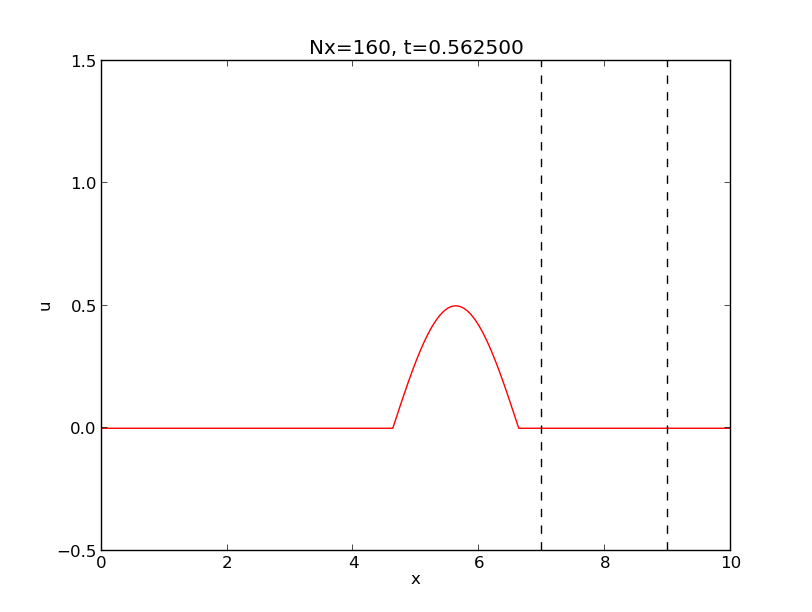
\includegraphics[width=0.9\linewidth]{testfigs/wave1D.png}}
  \caption{
  Visualization \textbf{of} a \emph{wave}. \label{fig:impact}
  }
\end{figure}
%\clearpage % flush figures fig:impact
Figures without captions are allowed and will be inlined.
\vspace{6mm}
% inline figure
\centerline{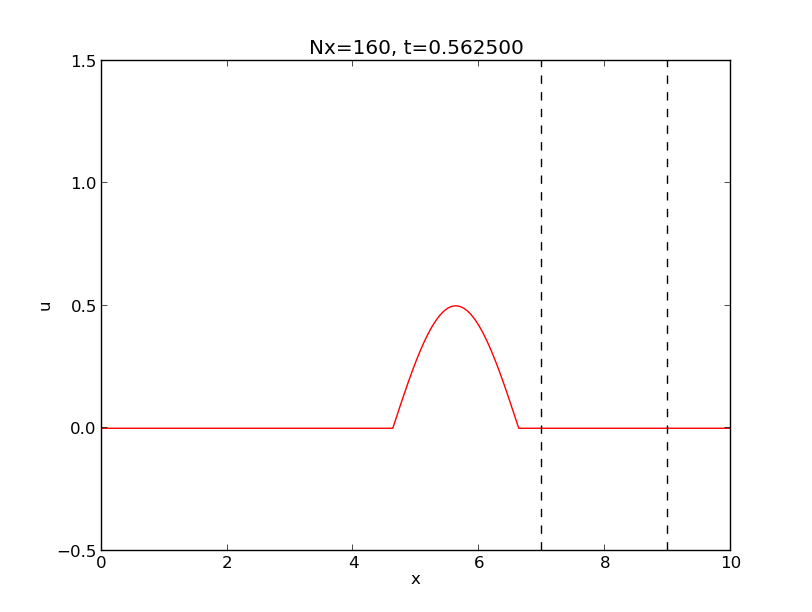
\includegraphics[width=0.9\linewidth]{testfigs/wave1D.png}}
\vspace{6mm}
\index{movies}
% Test multi-line caption in figure with sidecap=True
Here is figure~\vref{myfig} with a long (illegal) multi-line caption
containing inline verbatim text:
\begin{SCfigure}
  \centering
  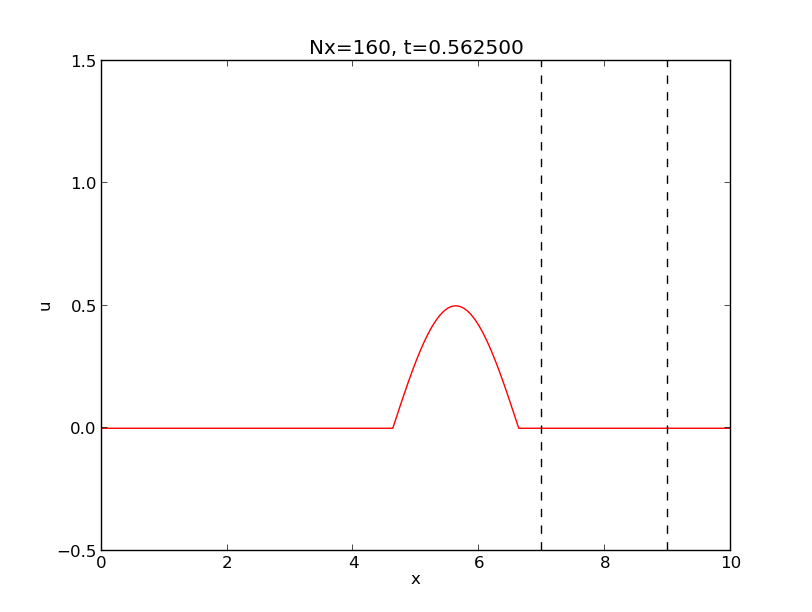
\includegraphics[width=0.9\linewidth]{testfigs/wave1D.png}
  \caption{
  A long caption spanning several lines and containing verbatim words like \protect \Verb!my\_file\_v1! and \protect \Verb!my\_file\_v2! as well as math with subscript as in $t_{i+1}$. \label{myfig}
  }
\end{SCfigure}
%\clearpage % flush figures myfig
% Must be a blank line after MOVIE or FIGURE to detect this problem
Test URL as figure name:
\vspace{6mm}
% inline figure
\centerline{\includegraphics[width=0.8\linewidth]{downloaded_figures/f_plot.png}}
\vspace{6mm}
% Test wikimedia type of files that otherwise reside in subdirs
\paragraph{Remark.}
Movies are tested in separate file \texttt{movies.do.txt}.
% Somewhat challenging heading with latex math, \t, \n, ? and parenthesis
\subsection{The $\theta$ parameter (not $\nabla$?)}
\label{decay:sec:theta}
Functions do not always need to be advanced, here is one
involving $\theta$:
\begin{cod}{cbg_blue1}\begin{lstlisting}[language=Python,style=myspeciallststyle,numbers=left,numberstyle=\tiny,stepnumber=3,numbersep=15pt,xleftmargin=1mm]
def f(theta):
    return theta**2

\end{lstlisting}\end{cod}
\noindent

\paragraph{More on $\theta$.}
Here is more text following headline with math.
Newcommands must also be tested in this \report:
$\half$, $\halfi$, $\x$, $\Ddt{u}$,
both inline and in block:
\begin{align}
\Ddt{u} &= 0\nonumber
\\ 
\half &= \halfi\\ 
\half\x &= \normalvec
\end{align}
Or with align with label and numbers:
\begin{align}
\Ddt{u} &= 0
\label{aligneq1}
\\ 
\half &= \halfi\\ 
\half\x &= \normalvec
\label{aligneq2}
\end{align}
% Must test more complicated align and matrix compositions
% where DocOnce inserts auto-numbered labels etc.
First one numbered (automatically):
\begin{align}
\begin{pmatrix}
G_2 + G_3 & -G_3 & -G_2 & 0 \\ 
-G_3 & G_3 + G_4 & 0 & -G_4 \\ 
-G_2 & 0 & G_1 + G_2 & 0 \\ 
0 & -G_4 & 0 & G_4
\end{pmatrix}
&=
\begin{pmatrix}
 v_1 \\ 
 v_2 \\ 
 v_3 \\ 
 v_4
\end{pmatrix}
+ \cdots \\ 
\begin{pmatrix}
 C_5 + C_6 & -C_6 & 0 & 0 \\ 
 -C_6 & C_6 & 0 & 0 \\ 
 0 & 0 & 0 & 0 \\ 
 0 & 0 & 0 & 0
\end{pmatrix}
  &= \frac{d}{dt}\begin{pmatrix}
 v_1 \\ 
 v_2 \\ 
 v_3 \\ 
 v_4
\end{pmatrix} +
\begin{pmatrix}
 0 \\ 
 0 \\ 
 0 \\ 
 -i_0
\end{pmatrix}
\nonumber
\end{align}
Second numbered (automatically):
\begin{align}
\begin{pmatrix}
G_1 + G_2\\ 
-G_3 & G_4
\end{pmatrix}
&=
\begin{pmatrix}
 v_1 \\ 
 v_2
\end{pmatrix}
+ \cdots\nonumber
\\ 
\left(\begin{array}{ll}
y & 2\\ 
2 & 1
\end{array}\right)
\left(\begin{array}{ll}
0 \\ x
\end{array}\right)
&= \begin{pmatrix}
A \\ B
\end{pmatrix}
\end{align}
Both numbered, with label by the user:
\begin{align}
\begin{pmatrix}
G_1 + G_2\\ 
-G_3 & G_4
\end{pmatrix}
&=
\begin{pmatrix}
 v_1 \\ 
 v_2
\end{pmatrix}
+ \cdots \label{mymatrix:eq1}
\\ 
\label{mymatrix:eq2}
\left(\begin{array}{ll}
y & 2\\ 
2 & 1
\end{array}\right)
\left(\begin{array}{ll}
0 \\ x
\end{array}\right)
&= \begin{pmatrix}
A \\ B
\end{pmatrix}
\end{align}
Now we refer to (\ref{mymatrix:eq1})-(\ref{mymatrix:eq2}).
\subsection{Custom Environments}
Here is an attempt to create a theorem environment via Mako
(for counting theorems) and comment lines to help replacing lines in
the \texttt{.tex} by proper begin-end {\LaTeX} environments for theorems.
Should look nice in most formats!
% begin theorem
\label{theorem:fundamental1}
\paragraph{Theorem 5.}
Let $a=1$ and $b=2$. Then $c=3$.
% end theorem
% begin proof
\paragraph{Proof.}
Since $c=a+b$, the result follows from straightforward addition.
$\Diamond$
% end proof
As we see, the proof of Theorem 5 is a modest
achievement.
\subsection{Tables}
\label{subsec:table}
\index{test index with verbatim text@test index with {\rm\texttt{verbatim text}} which is possible}
\index{test two@test {\rm\texttt{two}} (separate) {\rm\texttt{verbatim expressions}} which is also possible}
\index{index with!subindex}
\index{\textbf{boldface word} in index}
\index{index with \textbf{boldface word}}
\index{index with!\textbf{boldface word} in subentry}
\index{double \textbf{boldface word}! \textbf{boldface word} in subentry too}
% index with comma could fool sphinx
\index{index, with comma, and one more}
Let us take this table from the manual:
\begin{table}
\caption{
Testing table environment in {\LaTeX}, enabled by testing on the "latex" format
with the preprocessor.
\label{mytab}
}
\begin{quote}
\begin{tabular}{lrr}
\hline
\multicolumn{1}{c}{ time } & \multicolumn{1}{c}{ velocity } & \multicolumn{1}{c}{ acceleration } \\
\hline
0.0  & 1.4186   & -5.01        \\
2.0  & 1.376512 & 11.919       \\
4.0  & 1.1E+1   & 14.717624    \\
\hline
\end{tabular}
\end{quote}
\noindent
\end{table}
The DocOnce source code reads
\begin{cod}{cbg_blue1}\begin{lstlisting}[language=Python,style=myspeciallststyle,numbers=left,numberstyle=\tiny,stepnumber=3,numbersep=15pt,xleftmargin=1mm]

  |--------------------------------|
  |time  | velocity | acceleration |
  |--l--------r-----------r--------|
  | 0.0  | 1.4186   | -5.01        |
  | 2.0  | 1.376512 | 11.919       |
  | 4.0  | 1.1E+1   | 14.717624    |
  |--------------------------------|


\end{lstlisting}\end{cod}
\noindent

Here is yet another table to test that we can handle more than
one table:
\begin{quote}
\begin{tabular}{lll}
\hline
\multicolumn{1}{l}{ time } & \multicolumn{1}{l}{ velocity } & \multicolumn{1}{l}{ acceleration } \\
\hline
0.0  & 1.4186   & -5.01        \\
1.0  & 1.376512 & 11.919       \\
3.0  & 1.1E+1   & 14.717624    \\
\hline
\end{tabular}
\end{quote}
\noindent
And one with math headings (that are expanded and must be treated
accordingly), verbatim heading and entry, and no space around the pipe
symbol:
\begin{quote}
\begin{tabular}{lrrr}
\hline
\multicolumn{1}{c}{ $i$ } & \multicolumn{1}{c}{ $h_i$ } & \multicolumn{1}{c}{ $\bar T_i$ } & \multicolumn{1}{c}{ \Verb!L\_i! } \\
\hline
0   & 0      & 288        & -0.0065    \\
1   & 11,000 & 216        & 0.0        \\
2   & 20,000 & 216        & 0.001      \\
3   & 32,000 & 228        & 0.0028     \\
4   & 47,000 & 270        & 0.0        \\
5   & 51,000 & 270        & -0.0028    \\
6   & 71,000 & 214        & \texttt{NaN} \\
\hline
\end{tabular}
\end{quote}
\noindent
And add one with verbatim headings (with underscores),
and rows starting with \texttt{|-} because of a negative number,
and \texttt{|} right before and after verbatim word (with no space):
\begin{quote}
\begin{tabular}{rrrr}
\hline
\multicolumn{1}{c}{ exact } & \multicolumn{1}{c}{ \Verb!v\_1! } & \multicolumn{1}{c}{ $a_i$ + \Verb!v\_2! } & \multicolumn{1}{c}{ \Verb!verb\_3\_! } \\
\hline
9     & 9.62       & 5.57               & 8.98           \\
-20   & -23.39     & -7.65              & -19.93         \\
10    & 17.74      & -4.50              & 9.96           \\
0     & -9.19      & 4.13               & -0.26          \\
\hline
\end{tabular}
\end{quote}
\noindent
Pipe symbols in verbatim and math text in tables used to pose difficulties,
but not
anymore:
\begin{quote}
\begin{tabular}{lr}
\hline
\multicolumn{1}{c}{ $S$ } & \multicolumn{1}{c}{ command } \\
\hline
$ ||a_0|| $ & \texttt{norm|length} \\
$x\cap y$   & \texttt{x|y}         \\
\hline
\end{tabular}
\end{quote}
\noindent
Here is a table with X alignment:
\begin{quote}
\begin{tabularx}{\linewidth}{cX}
\hline
\multicolumn{1}{c}{ Type } & \multicolumn{1}{c}{ Description } \\
\hline
X     & Alignment character that is used for specifying a potentially very long text in a column in a table. It makes use of the \texttt{tabularx} package in {\LaTeX}, otherwise (for other formats) it means \texttt{l} (centered alignment). \\
l,r,c & standard alignment characters                                                                                                                                                                                                       \\
\hline
\end{tabularx}
\end{quote}
\noindent
Finally, a table with math
and URLs.
% Mako code to expand URLs in the table
% (These types of tables did not work before Jan 2014)
\begin{quote}
\begin{tabular}{ccc}
\hline
 \\
\hline
$\mathcal{L}=0$         & 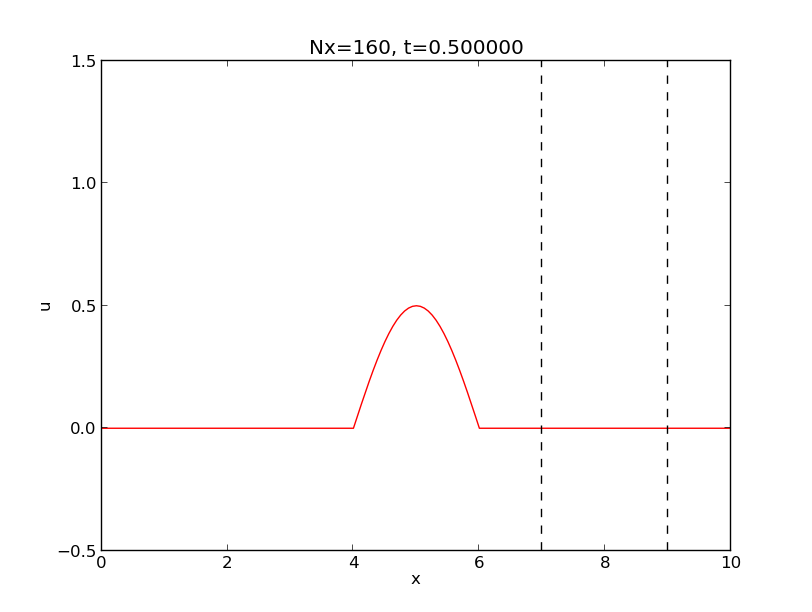
\includegraphics[width=2cm]{../doc/src/manual/mov/wave_frames/frame_0080.png} & 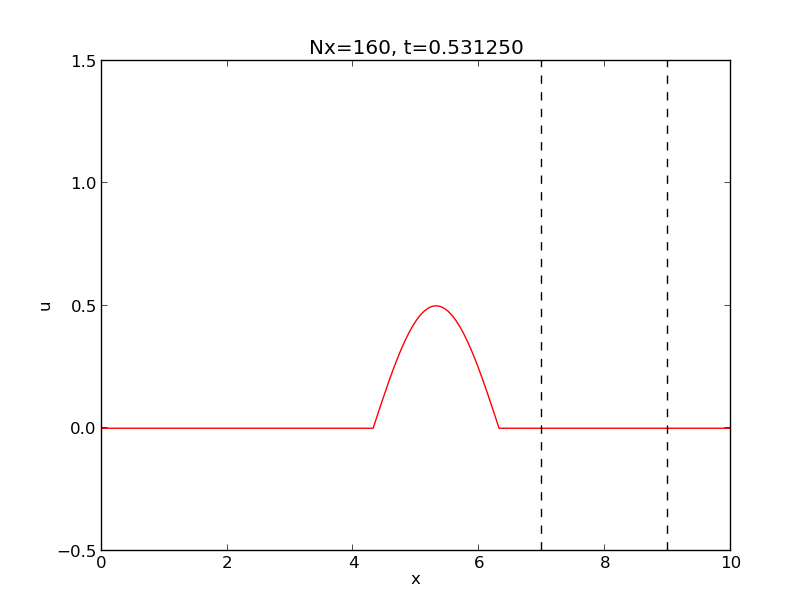
\includegraphics[width=2cm]{../doc/src/manual/mov/wave_frames/frame_0085.png} \\
$a=b$                   & 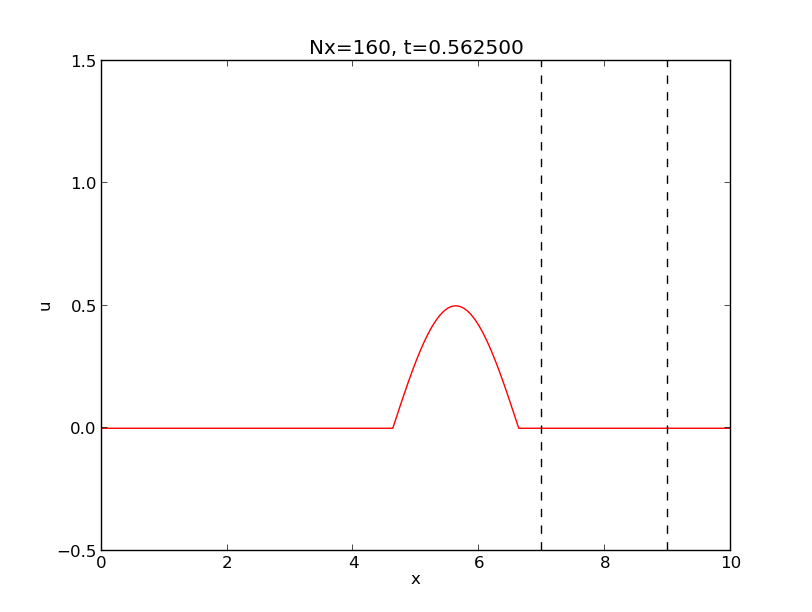
\includegraphics[width=2cm]{../doc/src/manual/mov/wave_frames/frame_0090.png} & 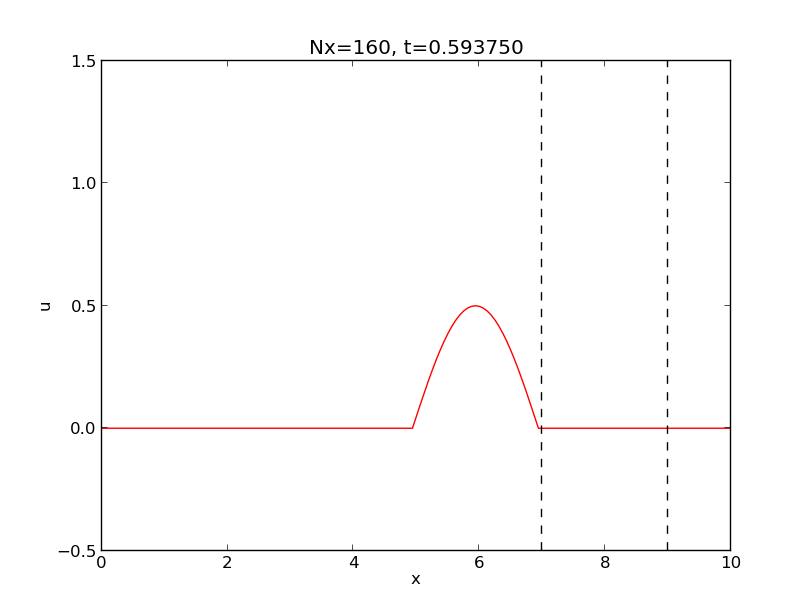
\includegraphics[width=2cm]{../doc/src/manual/mov/wave_frames/frame_0095.png} \\
$\nabla\cdot\bm{u} =0 $ & 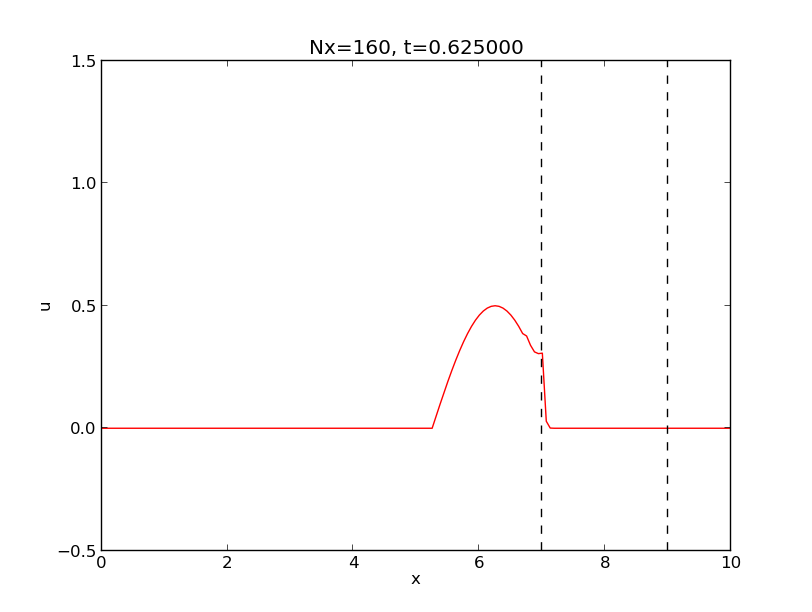
\includegraphics[width=2cm]{../doc/src/manual/mov/wave_frames/frame_0100.png} & 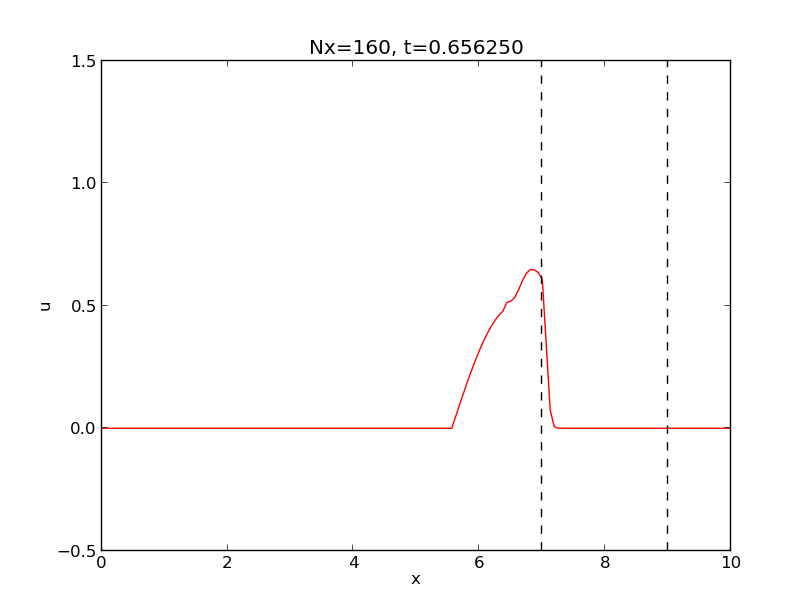
\includegraphics[width=2cm]{../doc/src/manual/mov/wave_frames/frame_0105.png} \\
\hline
\end{tabular}
\end{quote}
\noindent
\subsection{A test of verbatim words in heading with subscript $a_i$: \protect\Verb!my\_file\_v1! and \protect\Verb!my\_file\_v2! }
\paragraph{Paragraph with verbatim and math: \protect\Verb!my\_file\_v1.py! and \protect\Verb!my\_file\_v2.py! define some math $a_{i-1}$.}
Here is more \Verb!__verbatim__! code and
some plain text on a new line.
% Test various types of headlines
\subsection{\textbf{Just bold}}
Some text.
\subsection{\emph{Just emphasize}}
Some text.
\subsection{\texttt{Just verbatim} }
Some text.
\subsection{\textbf{Bold} beginning}
Some text.
\subsection{\emph{Emphasize} beginning}
Some text.
\subsection{\texttt{Verbatim} beginning}
Some text.
\subsection{Maybe \textbf{bold end}}
Some text.
\subsection{Maybe \emph{emphasize end}}
Some text.
\subsection{Maybe \texttt{verbatim end} }
Some text.
\subsection{The middle has \textbf{bold} word}
Some text.
\subsection{The middle has \emph{emphasize} word}
Some text.
\subsection{The middle has \texttt{verbatim} word}
Some text.
\paragraph{\emph{Just emphasize}.}
Some text.
\paragraph{\texttt{Just verbatim}.}
Some text.
\paragraph{\emph{Emphasize} beginning.}
Some text.
\paragraph{\texttt{Verbatim beginning}.}
Some text.
\paragraph{Maybe \emph{emphasize end}.}
Some text.
\paragraph{Maybe \texttt{verbatim end}.}
Some text.
\paragraph{The middle has \emph{emphasize} word.}
Some text.
\paragraph{The middle has \texttt{verbatim} word.}
Some text.
\paragraph{Ampersand.}
We can test Hennes {\&} Mauritz, often abbreviated H{\&}M, but written
as \Verb!Hennes & Mauritz! and \Verb!H & M!.
A sole \Verb!&! must also work.
% Note: substitutions must not occur inside verbatim, just in ordinary text.
\begin{cod}{cbg_blue1}\begin{lstlisting}[language=Python,style=myspeciallststyle,numbers=left,numberstyle=\tiny,stepnumber=3,numbersep=15pt,xleftmargin=1mm]
# Just to check that ampersand works in code blocks:
c = a & b

\end{lstlisting}\end{cod}
\noindent

\paragraph{Quotes.}
Let us also add a test of quotes such as ``double quotes, with numbers
like 3.14 and newline/comma and hyphen (as in double-quote)''; written
in the standard LaTeX-style that gives correct {\LaTeX} formatting and
ordinary double quotes for all non-LaTeX formats.  Here is another
sentence that ``caused'' a bug in the past because double backtick
quotes could imply verbatim text up to a verbatim word starting with
period, like \texttt{.txt}.
More quotes to be tested for spellcheck:
(``with parenthesis''), ``with newline''
and ``with comma'', ``hyphen''-wise, and ``period''.
\subsection{Bibliography test}
Here is an example: \cite{Langtangen_Pedersen_2002} discussed propagation of
large destructive water waves, \cite{Langtangen_et_al_2002} gave
an overview of numerical methods for solving the Navier--Stokes equations,
while the use of Backward Kolmogorov equations for analyzing
random vibrations was investigated in \cite{Langtangen_1994a}.
The book chapter \cite{Mardal_et_al_2003a} contains information on
C++ software tools for programming multigrid methods. A real retro
reference is \cite{Langtangen_1988d} about a big FORTRAN package.
Multiple references are also possible, e.g., see
\cite{Langtangen_Pedersen_2002,Mardal_et_al_2003a}.
We need to cite more than 10 papers to reproduce an old formatting
problem with blanks in the keys in reST format:
\cite{Langtangen_1992c,Langtangen_1994a,Mortensen_et_al_2011,Langtangen_Pedersen_2002}
and
\cite{Langtangen_et_al_2002,Glimsdal_et_al_20006,Rahman_et_al_2006b,Haga_et_al_2011a,Langtangen_2003a,Langtangen_2008a,Langtangen:95}
and all the work of
\cite{Langtangen_2012,Mardal_et_al_2003a,Jeberg_et_al_2004} as well as
old work \cite{Langtangen_1988d} and \cite{Langtangen_1989e}, and the
talk \cite{Langtangen_talk_2007a}.
Langtangen also had two thesis \cite{Langtangen:85,Langtangen_1989e}
back in the days.
More retro citations are
the old ME-IN323 book \cite{Langtangen:91} and the
\cite{Langtangen:94b} OONSKI '94 paper.
% --- begin exercise ---
\begin{doconceexercise}
\refstepcounter{doconceexercisecounter}
\exercisesection{Example \thedoconceexercisecounter: Examples can be typeset as exercises}
                             
\label{Example}
Examples can start with a subsection heading starting with \texttt{Example:}
and then, with the command-line option \Verb!--examples_as_exercises! be
typeset as exercises. This is useful if one has solution
environments as part of the example.
\subex{a)}
State some problem.
\paragraph{Solution.}
The answer to this subproblem can be written here.
\subex{b)}
State some other problem.
\paragraph{Hint 1.}
A hint can be given.
\paragraph{Hint 2.}
Maybe even another hint?
\paragraph{Solution.}
The answer to this other subproblem goes here,
maybe over multiple doconce input lines.
\end{doconceexercise}
% --- end exercise ---
\subsection{User-defined environments}
Example~\vref{ex:test:1p1} demonstrates how to write a test function.
That is, a special test function for a function \texttt{add} appears in
Example~\vref{ex:test:1p1}.
\begin{example}
\label{ex:test:1p1}
\noindent\emph{A test function}.
Suppose we want to write a test function for checking the
implementation of a Python function for addition.
\begin{cod}{cbg_blue1}\begin{lstlisting}[language=Python,style=myspeciallststyle,numbers=left,numberstyle=\tiny,stepnumber=3,numbersep=15pt,xleftmargin=1mm]
def add(a, b):
    return a + b

def test_add():
    a = 1; b = 1
    expected = a + b
    computed = add(a, b)
    assert expected == computed

\end{lstlisting}\end{cod}
\noindent

\end{example}
\begin{example}
\label{ex:math:1p1}
\noindent\emph{Addition}.
We have
\[ 1 + 1 = 2 \]
or in tabular form:
\begin{quote}
\begin{tabular}{cc}
\hline
\multicolumn{1}{c}{ Problem } & \multicolumn{1}{c}{ Result } \\
\hline
$1+1$   & $2$    \\
\hline
\end{tabular}
\end{quote}
\noindent
\end{example}
\begin{tcolorbox}[%skin=widget,
boxrule=1mm,
coltitle=black,
colframe=blue!45!white,
colback=blue!15!white,
width=(.9\linewidth),before=\hfill,after=\hfill,
adjusted title={Highlight box!}]
This environment is used to highlight something:
\[ E = mc^2 \]
\end{tcolorbox}
\subsection{URLs}
\label{subsubsec:ex}
Testing of URLs: hpl's home page \href{{https://folk.uio.no/hpl}}{hpl}, or
the entire URL if desired, \href{{https://folk.uio.no/hpl}}{\nolinkurl{https://folk.uio.no/hpl}}.  Here is a
plain file link \href{{testdoc.do.txt}}{\nolinkurl{testdoc.do.txt}}, or \href{{testdoc.do.txt}}{\nolinkurl{testdoc.do.txt}}, or
\href{{testdoc.do.txt}}{\nolinkurl{testdoc.do.txt}} or \href{{testdoc.do.txt}}{\nolinkurl{testdoc.do.txt}} or \href{{testdoc.do.txt}}{a link with
newline}. Can test spaces with the link with word
too: \href{{https://folk.uio.no/hpl}}{hpl} or \href{{https://folk.uio.no/hpl}}{hpl}. Also \texttt{file:///} works: \href{{file:///home/hpl/vc/doconce/doc/demos/manual/manual.html}}{link to a
file} is
fine to have. Moreover, ``loose'' URLs work, i.e., no quotes, just
the plain URL as in \href{{https://folk.uio.no/hpl}}{\nolinkurl{https://folk.uio.no/hpl}}, if followed by space, comma,
colon, semi-colon, question mark, exclamation mark, but not a period
(which gets confused with the periods inside the URL).
Mail addresses can also be used: \href{{mailto:hpl@simula.no}}{\nolinkurl{hpl@simula.no}}, or just a \href{{mailto:hpl@simula.no}}{mail link}, or a raw \href{{mailto:hpl@simula.no}}{\nolinkurl{mailto:hpl@simula.no}}.
Here are some tough tests of URLs, especially for the \texttt{latex} format:
\href{{https://en.wikipedia.org/wiki/Newton%E2%80%93Cotes_formulas}}{Newton-Cotes} formulas
and a \href{{https://www.springer.com/mathematics/computational+science+%26+engineering/book/978-3-642-23098-1}}{good book}. Need to test
Newton-Cotes with percentage in URL too:
\href{{https://en.wikipedia.org/wiki/Newton%E2%80%93Cotes_formulas}}{\nolinkurl{https://en.wikipedia.org/wiki/Newton\%E2\%80\%93Cotes_formulas}}
and \href{{https://en.wikipedia.org/wiki/Newton-Cotes#Open_Newton.E2.80.93Cotes_formulae}}{\nolinkurl{https://en.wikipedia.org/wiki/Newton-Cotes\#Open_Newton.E2.80.93Cotes_formulae}} which has a shebang.
For the \texttt{--device=paper} option it is important to test that URLs with
monospace font link text get a footnote
(unless the \Verb!--latex_no_program_footnotelink!
is used), as in this reference to
\href{{https://github.com/hplgit/INF5620/tree/gh-pages/src/decay/experiments/decay_mod.py}}{\nolinkurl{decay_mod}}, \href{{https://tinyurl.com/pwyasaa/formulas.ball1.py}}{\nolinkurl{ball1.py}},
and \href{{https://tinyurl.com/pwyasaa/formulas.ball2.py}}{\nolinkurl{ball2.py}}.
% Comments should be inserted outside paragraphs (because in the rst
% format extra blanks make a paragraph break).
% Note that when there is no https: or file:, it can be a file link
% if the link name is URL, url, "URL", or "url". Such files should,
% if rst output is desired, but placed in a \Verb!_static*! folder.
More tough tests: repeated URLs whose footnotes when using the
\texttt{--device=paper} option must be correct. We have
\href{{https://google.com}}{google}, \href{{https://google.com}}{google}, and
\href{{https://google.com}}{google}, which should result in exactly three
footnotes.
\subsection{Test of Some {\LaTeX} Fixes}
Let's check abbr.~of some common kind, e.g.~the well-known i.e.
expression as an example, and 1 vs.~2 which is also often used.
Dr.~Tang and Prof.~Monsen, or maybe also prof.~Ting,
will go to the Dept.~of Science to test how Mr.~Hansen is doing together
with Ms.~Larsen. A reference like Sec.~\vref{subsubsec:ex} or
Ch.~\vref{subsubsec:ex}, or even App.~\vref{subsubsec:ex}, must also be
handled. Likewise, this is test no.~$i$ of DocOnce features.
Also, look at Fig.~4 to see how the data compares with Tab.~\vref{mytab}.
Percentage must be fixed: 7\%,  87.65\% and
50\% at the beginning of the line.
% !split and check if these extra words are included properly in the comment
\section{{\LaTeX} Mathematics}
Here is an equation without label using backslash-bracket environment:
\[ a = b + c \]
or with number and label, as in (\ref{my:eq1}), using the equation environment:
\begin{equation}
{\partial u\over\partial t} = \nabla^2 u \label{my:eq1}
\end{equation}
We can refer to this equation by (\ref{my:eq1}).
Here is a system without equation numbers, using the align-asterisk environment:
\begin{align*}
\pmb{a} &= \pmb{q}\times\pmb{n} \\ 
b &= \nabla^2 u + \nabla^4 v
\end{align*}
And here is a system of equations with labels in an align environment:
\begin{align}
a &= q + 4 + 5+ 6 \label{eq1} \\ 
b &= \nabla^2 u + \nabla^4 x \label{eq2}
\end{align}
We can refer to (\ref{eq1})-(\ref{eq2}). They are a bit simpler than
the Navier--Stokes equations. And test {\LaTeX} hyphen in \texttt{CG-2}.
Also test $a_{i-j}$ as well as $kx-wt$.
Testing \texttt{alignat} environment:
\begin{alignat}{2}
a &= q + 4 + 5+ 6\qquad & \mbox{for } q\geq 0 \label{eq1a} \\ 
b &= \nabla^2 u + \nabla^4 x & x\in\Omega \label{eq2a}
\end{alignat}
Many of the next environments will fail in non-latex formats.
Testing multiline:
\begin{multline}
a = b = q + \\ 
  f + \nabla\cdot\nabla u
\label{multiline:eq1}
\end{multline}
Testing split:
\begin{equation}
\label{split:envir:eq}
\begin{split}
a = b = q &+ \\ 
  & f + \nabla\cdot\nabla u
\end{split}
\end{equation}
We can refer to the last equation by (\ref{split:envir:eq}).
Testing gather:
\begin{gather}
a = b \\ 
c = d + 7 + 9
\end{gather}
Let us refer to (\ref{eq1})-(\ref{eq2}) again, and to the
alignat variant (\ref{eq1a})-(\ref{eq2a}), and to (\ref{my:eq1}).
Testing eqnarray:
\begin{eqnarray}
{\partial u\over\partial t} &=& \nabla^2 u + f, \label{myeq1}\\ 
{\partial v\over\partial t} &=& \nabla\cdot(q(u)\nabla v) + g \label{myeq2}
\end{eqnarray}
More mathematical typesetting is demonstrated in the coming exercises.
Below, we have Problem~\vref{demo:ex:1} and Project~\vref{demo:ex:2},
as well as Projects~\vref{proj:circle1} and~\vref{exer:you}, and in
between there we have Exercise~\vref{exer:some:formula}.
\section{Exercises}
% --- begin exercise ---
\begin{doconceexercise}
\refstepcounter{doconceexercisecounter}
\exercisesection{Problem \thedoconceexercisecounter: Flip a Coin}
                             
\label{demo:ex:1}
% keywords = random numbers; Monte Carlo simulation; ipynb
% Torture tests
\subex{a)}
Make a program that simulates flipping a coin $N$ times.
Print out ``tail'' or ``head'' for each flip and
let the program count the number of heads.
% --- begin hint in exercise ---
\paragraph{Hint 1.}
Use \texttt{r = random.random()} and define head as \texttt{r <= 0.5}.
% --- end hint in exercise ---
% --- begin hint in exercise ---
\paragraph{Hint 2.}
Draw an integer among $\{1,2\}$ with
\texttt{r = random.randint(1,2)} and define head when \texttt{r} is 1.
% --- end hint in exercise ---
% --- begin answer of exercise ---
\paragraph{Answer.}
If the \texttt{random.random()} function returns a number $<1/2$, let it be
head, otherwise tail. Repeat this $N$ number of times.
% --- end answer of exercise ---
% --- begin solution of exercise ---
\paragraph{Solution.}
\begin{cod}{cbg_blue1}\begin{lstlisting}[language=Python,style=myspeciallststyle,numbers=left,numberstyle=\tiny,stepnumber=3,numbersep=15pt,xleftmargin=1mm]
import sys, random
N = int(sys.argv[1])
heads = 0
for i in range(N):
    r = random.random()
    if r <= 0.5:
        heads += 1
print('Flipping a coin %d times gave %d heads' % (N, heads))

\end{lstlisting}\end{cod}
\noindent

% --- end solution of exercise ---
\subex{b)}
Vectorize the code in a) using boolean indexing.
Vectorized code can be written in many ways.
Sometimes the code is less intuitive, sometimes not.
At least there is not much to find in Section~\vref{sec1}.
\subex{c)}
Vectorize the code in a) using \texttt{numpy.sum}.
% --- begin answer of exercise ---
\paragraph{Answer.}
\texttt{np.sum(np.where(r <= 0.5, 1, 0))} or \texttt{np.sum(r <= 0.5)}.
% --- end answer of exercise ---
In this latter subexercise, we have an
example where the code is easy to read.
\paragraph{My remarks.}
Remarks with such a subsubsection is treated as more text
after the last subexercise. Test a list too:
\begin{enumerate}
\item Mark 1.
\item Mark 2.
\end{enumerate}
\noindent
\noindent Filenames: \Verb!flip_coin.py!, \Verb!flip_coin.pdf!.
% Closing remarks for this Problem
\paragraph{Remarks.}
These are the exercise remarks, appearing at the very end.
% solution files: mysol.txt, mysol_flip_coin.py, yet_another.file
\end{doconceexercise}
% --- end exercise ---
\subsection{Not an exercise}
Should be possible to stick a normal section in the middle of many
exercises.
% --- begin exercise ---
\begin{doconceexercise}
\refstepcounter{doconceexercisecounter}
\exercisesection{Exercise \thedoconceexercisecounter: Test of plain text exercise}
                             
\label{my:exer1}
Very short exercise. What is the capital
of Norway?
\noindent Filename: \texttt{myexer1}.
\end{doconceexercise}
% --- end exercise ---
% --- begin exercise ---
\begin{doconceexercise}
\refstepcounter{doconceexercisecounter}
\exercisesection{Project \thedoconceexercisecounter: Compute a Probability}
                             
\label{demo:ex:2}
% Minimalistic exercise
What is the probability of getting a number between 0.5 and 0.6 when
drawing uniformly distributed random numbers from the interval $[0,1)$?
At the end we have a list because that caused problems in {\LaTeX}
in previous DocOnce versions:
\begin{enumerate}
\item item1
\item item2
\end{enumerate}
\noindent
% --- begin hint in exercise ---
\paragraph{Hint.}
To answer this question empirically, let a program
draw $N$ such random numbers using Python's standard \texttt{random} module,
count how many of them, $M$, that fall in the interval $(0.5,0.6)$, and
compute the probability as $M/N$.
% --- end hint in exercise ---
\end{doconceexercise}
% --- end exercise ---
% --- begin exercise ---
\begin{doconceexercise}
\refstepcounter{doconceexercisecounter}
\exercisesection{Project \thedoconceexercisecounter: Explore Distributions of Random Circles}
                             
\label{proj:circle1}
% keywords = ipynb
The formula for a circle is given by
\begin{align}
x &= x_0 + R\cos 2\pi t,
\label{circle:x}\\ 
y &= y_0 + R\sin 2\pi t,
\label{circle:y}
\end{align}
where $R$ is the radius of the circle, $(x_0,y_0)$ is the
center point, and $t$ is a parameter in the unit interval $[0,1]$.
For any $t$, $(x,y)$ computed from (\ref{circle:x})-(\ref{circle:y})
is a point on the circle.
The formula can be used to generate \texttt{n} points on a circle:
\begin{pro}{cbg_blue1}{bar_blue1}\begin{lstlisting}[language=Python,style=myspeciallststyle,numbers=left,numberstyle=\tiny,stepnumber=3,numbersep=15pt,xleftmargin=1mm]
import numpy as np

def circle(R, x0, y0, n=501):
    t = np.linspace(0, 1, n)
    x = x0 + R*np.cos(2*np.pi*t)
    y = y0 + R*np.sin(2*np.pi*t)
    return x, y

x, y = circle(2.0, 0, 0)

\end{lstlisting}\end{pro}
\noindent

% Often in an exercise we have some comments about the solution
% which we normally want to keep where they are.
The goal of this project is to draw $N$ circles with random
center and radius. Plot each circle using the \texttt{circle} function
above.
\subex{a)}
Let $R$ be normally distributed and $(x_0,y_0)$ uniformly distributed.
% --- begin hint in exercise ---
\paragraph{Hint.}
Use the \texttt{numpy.random} module to draw the
$x_0$, $y_0$, and $R$ quantities.
% --- end hint in exercise ---
% --- begin answer of exercise ---
\paragraph{Answer.}
Here goes the short answer to part a).
% --- end answer of exercise ---
% --- begin solution of exercise ---
\paragraph{Solution.}
Here goes a full solution to part a).
% --- end solution of exercise ---
\subex{b)}
Let $R$ be uniformly distributed and $(x_0,y_0)$ normally distributed.
\noindent Filename: \texttt{norm}.
\subex{c)}
Let $R$ and $(x_0,y_0)$ be normally distributed.
\noindent Filename: \texttt{circles}.
% Closing remarks for this Project
\paragraph{Remarks.}
At the very end of the exercise it may be appropriate to summarize
and give some perspectives.
\end{doconceexercise}
% --- end exercise ---
% --- begin exercise ---
\begin{doconceexercise}
\refstepcounter{doconceexercisecounter}
\exercisesection{Exercise \thedoconceexercisecounter: Determine some Distance}
                             
\label{exer:dist}
Intro to this exercise. Questions are in subexercises below.
% --- begin solution of exercise ---
\paragraph{Solution.}
Here goes a full solution of the whole exercise.
With some math $a=b$ in this solution:
\[ \hbox{math in solution: } a = b \]
And code \texttt{a=b} in this solution:
\begin{cod}{cbg_blue1}\begin{lstlisting}[language=Python,style=myspeciallststyle,numbers=left,numberstyle=\tiny,stepnumber=3,numbersep=15pt,xleftmargin=1mm]
a = b  # code in solution

\end{lstlisting}\end{cod}
\noindent

End of solution is here.
% --- end solution of exercise ---
\subex{a)}
Subexercises are numbered a), b), etc.
% --- begin hint in exercise ---
\paragraph{Hint 1.}
First hint to subexercise a).
With math $a=b$ in hint:
\[ a=b. \]
And with code (in plain verbatim) returning $x+1$ in hint:
\begin{cod}{cbg_blue1}\begin{lstlisting}[language=Python,style=myspeciallststyle,numbers=left,numberstyle=\tiny,stepnumber=3,numbersep=15pt,xleftmargin=1mm]
def func(x):
    return x + 1  # with code in hint

\end{lstlisting}\end{cod}
\noindent

% --- end hint in exercise ---
% --- begin hint in exercise ---
\paragraph{Hint 2.}
Second hint to subexercise a).
Test list in hint:
\begin{enumerate}
\item item1
\item item2
\end{enumerate}
\noindent
% --- end hint in exercise ---
\noindent Filename: \Verb!subexer_a.pdf!.
% --- begin answer of exercise ---
\paragraph{Answer.}
Short answer to subexercise a).
With math in answer: $a=b$.
% --- end answer of exercise ---
\subex{b)}
Here goes the text for subexercise b).
Some math $\cos^2 x + \sin^2 x = 1$ written one a single line:
\[ \cos^2 x + \sin^2 x = 1 \thinspace .\]
% --- begin hint in exercise ---
\paragraph{Hint.}
A hint for this subexercise.
% --- end hint in exercise ---
\noindent Filename: \Verb!subexer_b.pdf!.
% --- begin solution of exercise ---
\paragraph{Solution.}
Here goes the solution of this subexercise.
% --- end solution of exercise ---
% No meaning in this weired test example:
The text here belongs to the main (intro) part of the exercise. Need
closing remarks to have text after subexercises.
Test list in exercise:
\begin{enumerate}
\item item1
\item item2
% Closing remarks for this Exercise
\end{enumerate}
\noindent
\paragraph{Remarks.}
Some final closing remarks, e.g., summarizing the main findings
and their implications in other problems can be made. These
remarks will appear at the end of the typeset exercise.
\end{doconceexercise}
% --- end exercise ---
% --- begin exercise ---
\begin{doconceexercise}
\exercisesection{Some exercise without the "Exercise:" prefix}
% Another minimalistic exercise
Just some text. And some math saying that $e^0=1$ on a single line,
to test that math block insertion is correct:
\[ \exp{(0)} = 1 \]
And a test that the code \texttt{lambda x: x+2} is correctly placed here:
\begin{cod}{cbg_blue1}\begin{lstlisting}[language=Python,style=myspeciallststyle,numbers=left,numberstyle=\tiny,stepnumber=3,numbersep=15pt,xleftmargin=1mm]
lambda x: x+2

\end{lstlisting}\end{cod}
\noindent

% Have some comments at the end of the exercise to see that
% the Filename: ... is written correctly.
\end{doconceexercise}
% --- end exercise ---
% --- begin exercise ---
\begin{doconceexercise}
\refstepcounter{doconceexercisecounter}
\exercisesection{Exercise \thedoconceexercisecounter: Solution of differential equation}
                             
\label{sec:this:exer:de}

\begin{doconcequiz}
\refstepcounter{doconcequizcounter}
\label{quiz:diff:eq1}


\noindent\textbf{\large SOlution of differential equation}

\noindent
Given
\[ \frac{dy}{dx} = -y(x),\quad y(0)=1 \]
What is the solution of this equation?

\vspace{2mm}

\textbf{A}. 
$y=e^{-y}$

\textbf{B}. 
$y=e^{y}$

\textbf{C}. 
\begin{cod}{cbg_blue1}\begin{lstlisting}[language=Python,style=myspeciallststyle,numbers=left,numberstyle=\tiny,stepnumber=3,numbersep=15pt,xleftmargin=1mm]
from math import exp
def f(x):
    return exp(x)

\end{lstlisting}\end{cod}
\noindent

\textbf{D}. 
The solution cannot be found because there is a derivative in the equation.

\textbf{E}. 
The equation is meaningless: an equation must be an equation
for $x$ or $y$, not a function $y(x)$.


% --- begin answer of exercise ---
\paragraph{Answer:} A.
% --- end answer of exercise ---

% --- begin solution of exercise ---
\noindent {\bf Solution:}\\


\textbf{A}: Right. 

\textbf{B}: Wrong. Almost, but the sign is wrong (note the minus!).

\textbf{C}: Wrong. Ooops, forgot a minus: \texttt{exp(-x)}, otherwise this Python code
must be considered as a good answer. It is more natural,
though, to write the solution to the problem
in mathematical notation:
\[ y(x) = e^{-y}.\]

\textbf{D}: Wrong. Equations with derivatives can be solved;
they are termed \emph{differential
equations}.

\textbf{E}: Wrong. Equations where the unknown is a function, as $y(x)$
here, are called \emph{differential equations}, and are solved by
special techniques.


% --- end solution of exercise ---


\vspace{3mm}

\end{doconcequiz}


\end{doconceexercise}
% --- end exercise ---
% --- begin exercise ---
\begin{doconceexercise}
\refstepcounter{doconceexercisecounter}
\exercisesection{Example \thedoconceexercisecounter: Just an example}
                             
% This example needs the --examples_as_exercises option, otherwise
% it is just typeset as it is written.
\subex{a)}
What is the capital of Norway?
\paragraph{Answer.}
Oslo.
\end{doconceexercise}
% --- end exercise ---
\section{Here goes another section}
With some text, before we continue with exercises.
\section{More Exercises}
% --- begin exercise ---
\begin{doconceexercise}
\refstepcounter{doconceexercisecounter}
\exercisesection{Exercise \thedoconceexercisecounter: Make references to projects and problems}
                             
\label{exer:some:formula}
% Test comments not at the end only
Pick a statement from Project~\vref{proj:circle1} or Problem~\vref{demo:ex:1}
and verify it.
Test list at the end of an exercise without other elements (like subexercise,
hint, etc.):
\begin{enumerate}
\item item1
\item item2
\end{enumerate}
\noindent
\noindent Filename: \Verb!verify_formula.py!.
\end{doconceexercise}
% --- end exercise ---
% --- begin exercise ---
\begin{doconceexercise}
\refstepcounter{doconceexercisecounter}
\exercisesection{Project \thedoconceexercisecounter: References to Project~\vref{demo:ex:2} in a heading works for pdflatex}
                             
\label{exer:you}
Refer to the previous exercise as Exercise~\vref{exer:some:formula},
the two before that as Projects~\vref{demo:ex:2} and~\vref{proj:circle1},
and this one as Project~\vref{exer:you}.
\noindent Filename: \Verb!selc_composed.pdf!.
\end{doconceexercise}
% --- end exercise ---
\bibliographystyle{plain}
\bibliography{papers}
\appendix
\section{Just for testing; part I}
\label{app1}
This is the first appendix.
\subsection{A subsection within an appendix}
Some text.
\section{Just for testing; part II}
\label{app2}
This is more stuff for an appendix.
\subsection{Appendix: Testing identical titles}
Without label.
\subsection{Appendix: Testing identical titles}
\label{test:title:id1}
With label.
\subsection{Appendix: Testing identical titles}
\label{test:title:id2}
What about inserting a quiz?

\begin{doconcequiz}
\refstepcounter{doconcequizcounter}
\label{quiz:2}


\noindent\textbf{\large Capital of Norway}
\paragraph{Fundamental test:}
What is the capital of Norway?

\vspace{2mm}

\textbf{A}. 
Stockholm

\textbf{B}. 
London

\textbf{C}. 
Oslo

\textbf{D}. 
Bergen


% --- begin answer of exercise ---
\paragraph{Answer:} C.
% --- end answer of exercise ---

% --- begin solution of exercise ---
\noindent {\bf Solution:}\\


\textbf{A}: Wrong. Stockholm is the capital of Sweden.

\textbf{B}: Wrong. 

\textbf{C}: Right. 

\textbf{D}: Wrong. Those from Bergen would claim so, but nobody else.


% --- end solution of exercise ---


\vspace{3mm}

\end{doconcequiz}


\subsection{Appendix: Testing identical titles}
Without label.

\begin{notice_mdfboxadmon}[Tip.]
Here is a tip or hint box, typeset as a notice box.
\end{notice_mdfboxadmon} % title: Tip.


\clearpage
Need a lot of text to surround the summary box.
Version control systems allow you to record the history of files
and share files among several computers and collaborators in a
professional way. File changes on one computer are updated or
merged with changes on another computer. Especially when working
with programs or technical reports it is essential
to have changes documented and to
ensure that every computer and person involved in the project
have the latest updates of the files.
Greg Wilson' excellent \href{{https://software-carpentry.org/2010/07/script-for-introduction-to-version-control/}}{Script for Introduction to Version Control} provides a more detailed motivation why you will benefit greatly
from using version control systems.

\begin{summary_mdfboxadmon}[Summary.]
\textbf{Bold remark:} Make some text with this summary.
Much testing in this document, otherwise stupid content.
Much testing in this document, otherwise stupid content.
Much testing in this document, otherwise stupid content.
Much testing in this document, otherwise stupid content.
Much testing in this document, otherwise stupid content.
Much testing in this document, otherwise stupid content.
Much testing in this document, otherwise stupid content.
Much testing in this document, otherwise stupid content.
Much testing in this document, otherwise stupid content.
\end{summary_mdfboxadmon} % title: Summary.


Projects that you want to share among several computers or project
workers are today most conveniently stored at some web site "in the
cloud" and updated through communication with that site. I strongly
recommend you to use such sites for all serious programming and
scientific writing work - and all other important files.
The simplest services for hosting project files are \href{{https://dropbox.com}}{Dropbox} and \href{{https://drive.google.com}}{Google Drive}.
It is very easy to get started with these systems, and they allow you
to share files among laptops and mobile units with as many users as
you want. The systems offer a kind of version control in that the
files are stored frequently (several times per minute), and you can go
back to previous versions for the last 30 days. However, it is
challenging  to find the right version from the past when there are
so many of them.
More seriously, when several people may edit files simultaneously, it
can be difficult detect who did what when, roll back to previous
versions, and to manually merge the edits when these are
incompatible. Then one needs more sophisticated tools than Dropbox or
Google Drive: project hosting services with true version control
systems.  The following text aims at providing you with the minimum
information to started with such systems. Numerous other tutorials
contain more comprehensive material and in-depth explanations of the
concepts and tools.
The idea with project hosting services is that you have the files
associated with a project in the cloud. Many people may share these
files.  Every time you want to work on the project you explicitly
update your version of the files, edit the files as you like, and
synchronize the files with the "master version" at the site where the
project is hosted.  If you at some point need to go back to a
version of the files at some particular point in the past,
this is an easy operation. You can also use tools to see
what various people have done with the files in the various versions.
All these services are very similar. Below we describe how you get
started with Bitbucket, GitHub, and Googlecode. Launchpad works very
similarly to the latter three. All the project hosting services have
excellent introductions available at their web sites, but the recipes
below are much shorter and aim at getting you started as quickly as
possible by concentrating on the most important need-to-know steps.
The Git tutorials we refer to later in this document contain more
detailed information and constitute of course very valuable readings
when you use version control systems every day. The point now is
to get started.
\subsection{Appendix: Testing inline comments}
% Names can be [ A-Za-z0-9_'+-]+
Projects that you want to share among several computers or project
workers are today most conveniently stored at some web site "in the
cloud" and updated through communication with that
site. \shortinlinecomment{hpl's semi opinion 1}{ not sure if in the cloud is understood by all. }{ not sure if in } I strongly recommend you to use such sites for all serious
programming and scientific writing work - and all other important
files.
The simplest services for hosting project files is Dropbox. \longinlinecomment{mp 2}{ Simply go to \href{{https://dropbox.com}}{\nolinkurl{https://dropbox.com}} and watch the video. It explains how files, like \texttt{myfile.py}, perhaps containing much math, like $\partial u/\partial t$, are easily communicated between machines. }{ Simply go to \href{{https://dropbox.com}}{\nolinkurl{https://dropbox.com}} } It
is very easy to get started with Dropbox, and it allows you to share
files among \textcolor{red}{(hpl 3:)} \replace{laptops and mobile units}{computers, tablets, and phones}.
% Test horizontal rule
------
% Coments for editing
First\textcolor{red}{, (\textbf{edit 4}: add comma)} consider a quantity $Q$. \textcolor{red}{(edit 5:)} \replace{To this end,}{We note that}
$Q>0$, because (\textbf{edit 6}:) \remove{a} negative \textcolor{red}{(edit 7:)} \replace{quantity is}{quantities are} (\textbf{edit 8}:) \remove{just} negative.  \textcolor{red}{ (\textbf{edit 9}:) This comes as no surprise.}
% Test tailored latex figure references with page number
Let us refer to Figure~\vref{fig:impact} again.
Test references in a list:
\begin{itemize}
 \item \vref{sec1}
 \item \vref{subsec1}
 \item \vref{fig:impact}
\end{itemize}
\noindent
\subsection{Appendix: Testing headings ending with \texttt{verbatim inline} }
The point here is to test 1) \texttt{verbatim} code in headings, and 2)
ending a heading with verbatim code as this triggers a special
case in {\LaTeX}.
We also test mdash---used as alternative to hyphen without spaces around,
or in quotes:

\begin{quote}
\emph{Fun is fun}.---Unknown.
\end{quote}

The ndash should also be tested -- as in the Hanson--Nilson equations
on page 277--278.
And finally, what about admons, quotes, and boxes? They are tested
in a separate document: \texttt{admon.do.txt}.
% ------------------- end of main content ---------------
% #ifdef PREAMBLE
\cleardoublepage\phantomsection  % trick to get correct link to Index
\printindex
\end{document}
% #endif
